\documentclass[11pt]{article}

\usepackage[margin=1in]{geometry}
\usepackage[T1]{fontenc}
\usepackage{lmodern}
\usepackage{microtype}
\usepackage{amsmath}
\usepackage{graphicx}
\usepackage{subcaption}
\usepackage{float}
\usepackage{xcolor}
\usepackage[format=plain, font=small, labelfont={bf,color=accent}, skip=6pt]{caption}
\usepackage{titlesec}
\usepackage[colorlinks=true, linkcolor=accent, citecolor=accent, urlcolor=accent,
            pdftitle={Analysis of the DIPF},
            pdfauthor={}]{hyperref}

\definecolor{accent}{RGB}{20,60,110}

\titleformat{\section}
  {\normalfont\Large\bfseries\color{accent}}{\thesection}{0.6em}{}
\titleformat{\subsection}
  {\normalfont\large\bfseries\color{accent!85!black}}{\thesubsection}{0.6em}{}
\titlespacing*{\section}{0pt}{1.0em}{0.5em}
\titlespacing*{\subsection}{0pt}{0.7em}{0.3em}

\setlength{\textfloatsep}{8pt plus 2pt minus 3pt}
\setlength{\intextsep}{6pt plus 2pt minus 2pt}
\setlength{\abovecaptionskip}{4pt}
\setlength{\belowcaptionskip}{2pt}
\setlength{\parskip}{0.3em}
\setlength{\abovedisplayskip}{6pt plus 2pt minus 3pt}
\setlength{\belowdisplayskip}{6pt plus 2pt minus 3pt}
\setlength{\abovedisplayshortskip}{4pt plus 2pt minus 2pt}
\setlength{\belowdisplayshortskip}{4pt plus 2pt minus 2pt}

\title{\textcolor{accent}{\textbf{Analysis of the Obstacle Potential Function}}}
\author{}
\date{}

\begin{document}
\maketitle
\vspace{-1.5em}

\vspace{1em}

\section{Potential Function}

\begin{equation}
    U_{obst} = \frac{\lambda (|\Delta v| / \Delta v_{max})}
    {k(\Delta x, \Delta y, \Delta v_x, \Delta v_y)}
    \label{eq:potential}
\end{equation}

\begin{equation}
    k(\Delta x, \Delta y, \Delta v_x, \Delta v_y) =
    \begin{cases}
        0, & \text{if } |\Delta y| < l \text{ and } |\Delta x| < w \\[4pt]
        \left(1 - \dfrac{w}{|\Delta x|}\right) \sqrt{\left(\dfrac{\Delta x}{\tau_x}\right)^2 + \left(\dfrac{\Delta y}{\tau_y}\right)^2}, & \text{if } |\Delta y| \leq \dfrac{l\,|\Delta x|}{w} \\[8pt]
        \left(1 - \dfrac{l}{|\Delta y|}\right) \sqrt{\left(\dfrac{\Delta x}{\tau_x}\right)^2 + \left(\dfrac{\Delta y}{\tau_y}\right)^2}, & \text{otherwise}
    \end{cases}
    \label{eq:k-prime}
\end{equation}

\begin{align}
    \tau(\Delta x, \Delta v_x) &= \frac{(1 + \alpha |\Delta v_x|) + (\alpha |\Delta v_x| - 1)\tanh(-\Delta x \Delta v_x)}{2}\,\tau_x \\
    \tau(\Delta y, \Delta v_y) &= \frac{(1 + \alpha |\Delta v_y|) + (\alpha |\Delta v_y| - 1)\tanh(-\Delta y \Delta v_y)}{2}\,\tau_y
\end{align}

\noindent
Here $\Delta x, \Delta y$ are the relative position wrt obstacle vehicle, $\Delta v_x, \Delta v_y$ the relative velocities wrt obstacle vehicle.

\subsection{Potential Field Plots}

\begin{figure}[H]
    \centering
    \begin{subfigure}[b]{0.32\textwidth}
        \centering
        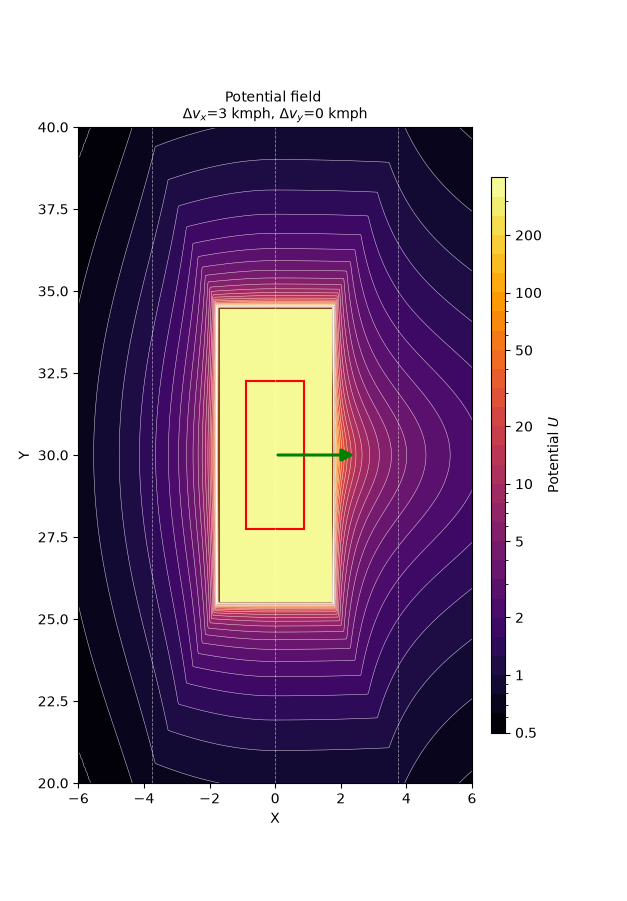
\includegraphics[width=\linewidth]{potential_vx.png}
        \caption{Varying $\Delta v_x$}
    \end{subfigure}
    \hfill
    \begin{subfigure}[b]{0.32\textwidth}
        \centering
        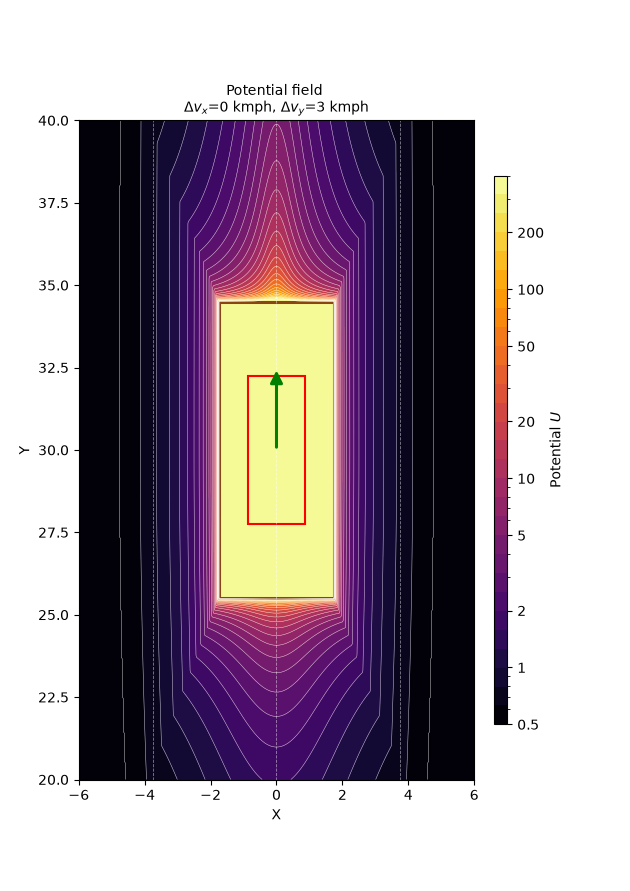
\includegraphics[width=\linewidth]{potential_vy.png}
        \caption{Varying $\Delta v_y$}
    \end{subfigure}
    \hfill
    \begin{subfigure}[b]{0.32\textwidth}
        \centering
        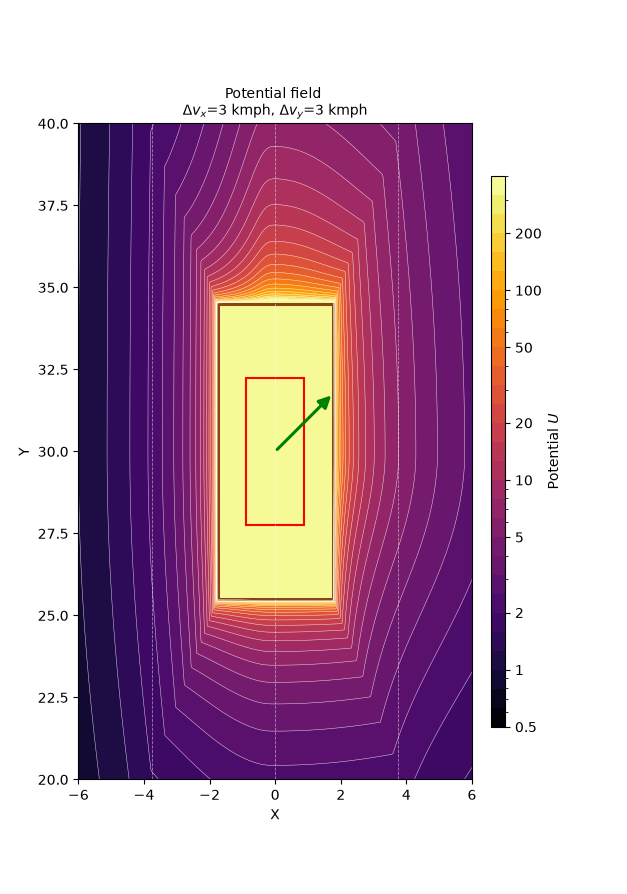
\includegraphics[width=\linewidth]{potential_vxvy.png}
        \caption{Varying $\Delta v_x, \Delta v_y$}
    \end{subfigure}
    \caption{Obstacle potential field $U_{obst}$.}
    \label{fig:potential-field}
\end{figure}

\subsection{Force Field}
\label{sec:force-field}
$$F=-\nabla U_{obst}$$
\begin{figure}[H]
    \centering
    \begin{subfigure}[b]{0.32\textwidth}
        \centering
        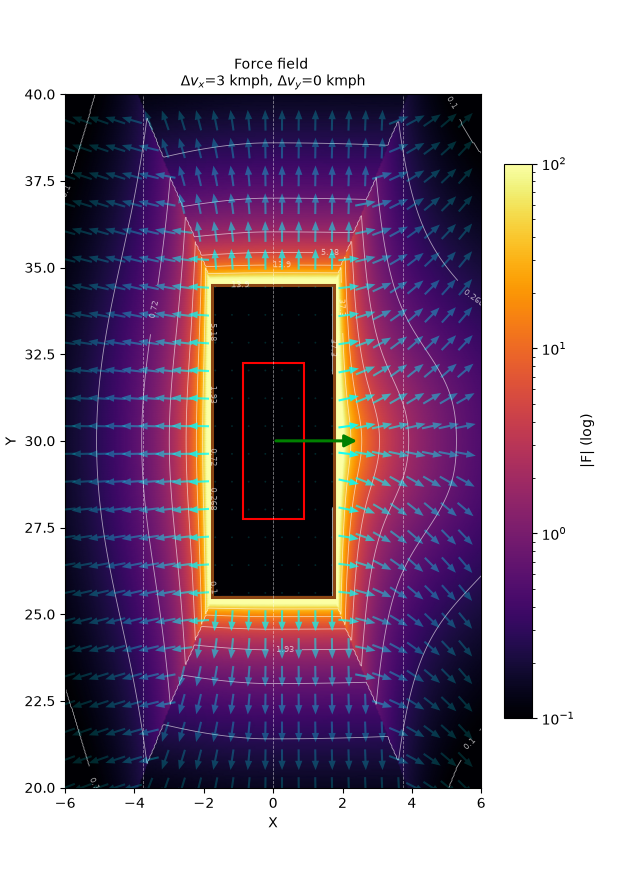
\includegraphics[width=\linewidth]{force_vx.png}
        \caption{Varying $\Delta v_x$}
        \label{fig:force-field-a}
    \end{subfigure}
    \hfill
    \begin{subfigure}[b]{0.32\textwidth}
        \centering
        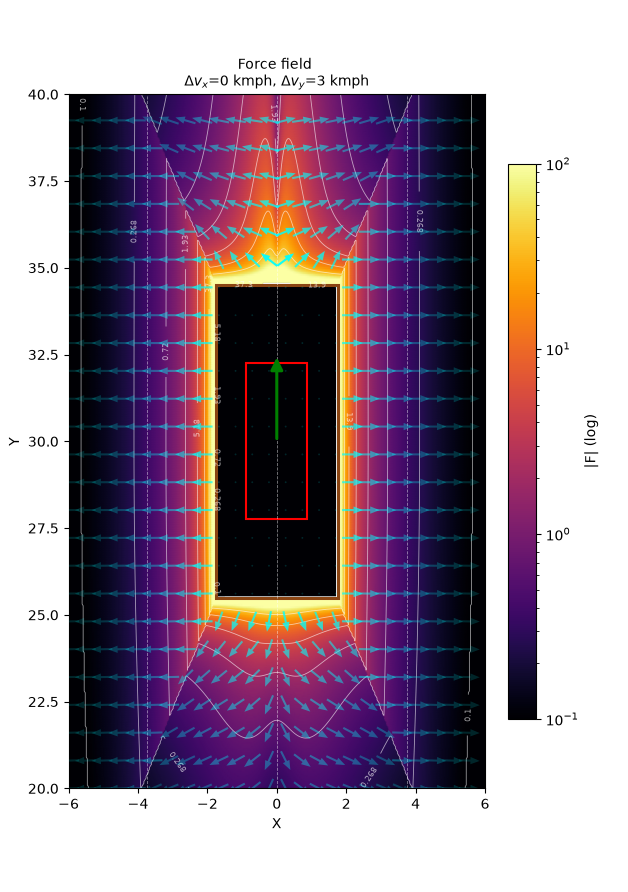
\includegraphics[width=\linewidth]{force_vy.png}
        \caption{Varying $\Delta v_y$}
        \label{fig:force-field-b}
    \end{subfigure}
    \hfill
    \begin{subfigure}[b]{0.32\textwidth}
        \centering
        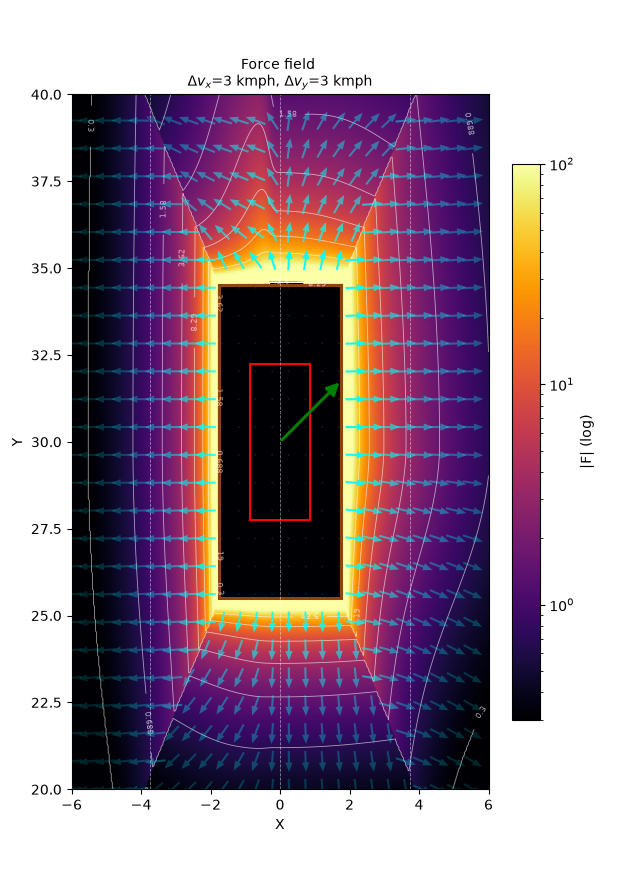
\includegraphics[width=\linewidth]{force_vxvy.png}
        \caption{Varying $\Delta v_x, \Delta v_y$}
        \label{fig:force-field-c}
    \end{subfigure}
    \caption{Force field derived from $U_{obst}$.}
    \label{fig:force-field}
\end{figure}
\newpage
\section{Possible Issues}

\subsection{Anomalous dip in the magnitude of force field}
\begin{figure}[H]
    \centering
    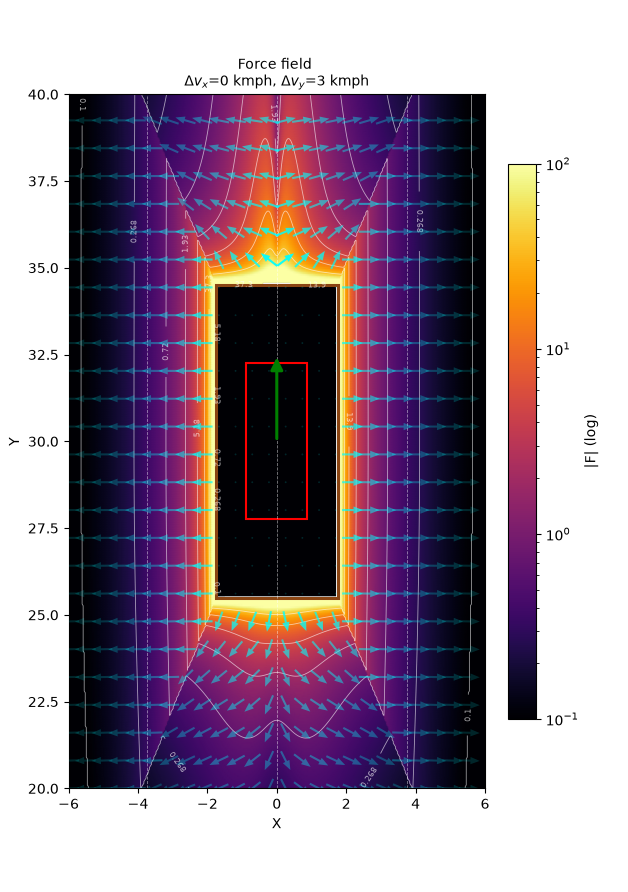
\includegraphics[width=0.5\textwidth]{force_vy.png}
\end{figure}
The magnitude of the force field dips near x=0 in the above plot which is undesirable  as the magnitude of force field should be maximum along x=0 when compared to the neighbouring points.
\subsection{Sensitivity to $\tau_x, \tau_y$ and Parallel Forces}

\begin{figure}[H]
    \centering
    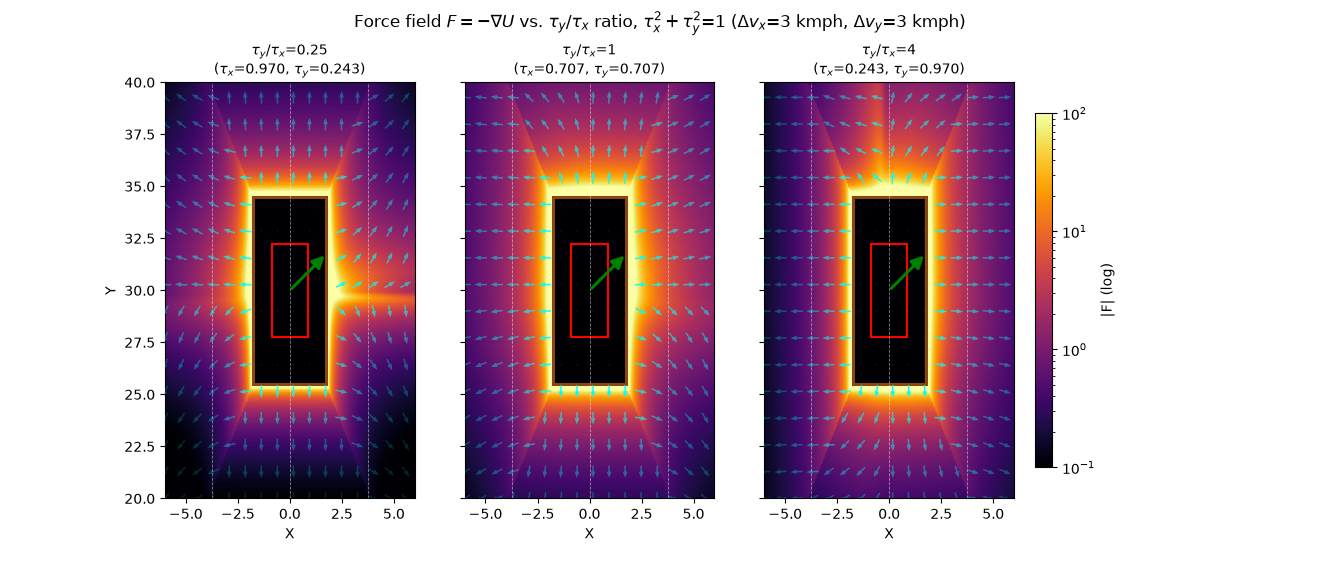
\includegraphics[width=1.0\textwidth]{tau_sensitivity.png}
    \caption{Sensitivity of the field to $\tau_x, \tau_y$.}
    \label{fig:tau-sensitivity}
\end{figure}
The shape of the potential is highly sensitive to $\tau_y/\tau_x$ and very high value or a very small value can cause the force field to be parallel in certain region which is not desirable.
\subsection{Velocity Behavior at a fixed point}

\begin{figure}[H]
    \centering
    
\includegraphics[width=0.6\textwidth]{base_vel.png}
    \caption{Velocity at a fixed point.}
    \label{fig:base-vel}
\end{figure}
The force increases with increase in receding velocity at a fixed point. In an ideal scenario the repulsive force should decrease when the vehicles are receding.
\subsection{More free parameters than DOF}

The model introduces 4 free parameters ($\lambda$, $\alpha$, $\tau_x$,
$\tau_y$) while the degree of freedom of the model is only 3. So reduction of parameters will help in the optimization problem.

\end{document}
